\documentclass[times,11pt,portrait]{article} %12pt, DOE SBIR/STTR

\usepackage[dvips]{graphicx}
%\usepackage[small,compact]{titlesec}
\usepackage{afterpage}

\usepackage{times}
\usepackage[dvips]{epsfig}
\usepackage{multirow}

\usepackage[usenames,dvipsnames]{color}

\usepackage[breaklinks=true,colorlinks,citecolor=blue,urlcolor=blue,linkcolor=blue]{hyperref}
\usepackage{breakurl}
%\usepackage{subfigure}
\usepackage{caption}
\usepackage{subcaption}

\usepackage{tweaklist} %used for globally changing enum and item spacing
\usepackage{natbib, natbibspacing}

\usepackage{algorithmic}
\usepackage[vlined,ruled]{algorithm2e}

%\usepackage{listings}
\usepackage{fancyvrb}
\newenvironment{CVerbatim}
 {\center\BVerbatim}
 {\endBVerbatim\endcenter}



\usepackage{titlesec}
%\usepackage{subfigure}
\usepackage[para]{footmisc}
\usepackage{hyperref}
\def\myurl#1{\setbox0\vbox{\hsize.5\maxdimen
\url{#1}\par
\global\setbox1\lastbox}\unhbox1 }



%\usepackage{titlesec}
\usepackage[small,compact]{titlesec}

\usepackage{vmargin}

\usepackage{wrapfig}
\setlength\hoffset{0in}
\setlength\voffset{-0.6in}
\setlength\oddsidemargin{-0.2in}
\setlength\evensidemargin{-0.2in}
\setlength\topmargin{0in}
\setlength\headheight{0.36in}
\setlength\headsep{0.05in}
\setlength\textheight{9.6in}
\setlength\textwidth{6.95in}
\setlength\marginparsep{0in}
\setlength\marginparwidth{0in}
\setlength\footskip{0.25in}

\usepackage{fancyhdr}
\pagestyle{fancy}


%% Setting up pagestyles for ``fancy''
%\chead{} % per section
\rhead{\bf{DOE SBIR FY2018.2 30.d Phase I Final Report}\\}
\lhead{{\bf RNET Technologies, Inc.}\\}

\renewcommand{\headrulewidth}{0.8pt}
\renewcommand{\footrulewidth}{0.5pt}

%\lfoot{\bf Proprietary Information}
\lfoot{}
\cfoot{\bf \thepage}
\rfoot{\bf 23$^rd$ April 2019} %due at 11:59pm ET

% Ensure pdflatex generates letter-size pdfs
\setpapersize{USletter}


\usepackage{vmargin}
% All proposals MUST use/include these margin and header settings.

% All proposals MUST use pdflatex and NOT latex/dvips/ps2pdf. Any
% changes to this must have approval from the RNET president and your
% manager. This is to ensure proper margins in all settings.

% ALWAYS use these margins unless the changes are discussed with RNET
% personnel.

%NOTE: When printing, you MUST ensure that ALL scaling is turned OFF
%for both the printer AND the Adobe settings. If Adobe scales the
%document, the printed margins will be WRONG (even if the PDF is
%correct).

% Please, always double check the margins by measuring the margins on the screen, either using a tool that gives a pixel offset of a pointer in a PDF or a ``screen tapemeasure''.

\usepackage[margin=1in]{geometry} % Used to ensure that PDF latex handles the
                      % length and margin settings
                      % approriately. http://en.wikibooks.org/wiki/LaTeX/Page_Layout

% Ensure pdflatex generates letter-size pdfs


% See http://en.wikibooks.org/wiki/LaTeX/Page_Layout for more
% information on dimensions. However, please do not change without proper
% approval.

\setlength\hoffset{0pt} 
\setlength\voffset{-1.05in} %need a header, so need to put the header in default 1'' maring
\setlength\oddsidemargin{0.0in} %leave 0
\setlength\evensidemargin{0.0in} %leave 0
\setlength\topmargin{0.2in}
\setlength\headheight{0.6in} 
\setlength\headsep{0.2in} 
\setlength\textheight{9.1in}
\setlength\textwidth{6.5in}
\setlength\marginparsep{0pt}
\setlength\marginparwidth{0in}
\setlength\footskip{0.35in}

\usepackage{fancyhdr}
\pagestyle{fancy}

% Ensure pdflatex generates letter-size pdfs
\setpapersize{USletter}


%\oddsidemargin -12pt \evensidemargin -12pt
%\topmargin -30pt \headheight 0.2in \headsep 0.0in \footheight 0.0in 
%\footskip 0.5in 

%\textheight 9.37in \textwidth 6.91in \columnsep .33in \columnseprule 0.0in
%\addtolength{\textheight}{2.2in}
%\addtolength{\textwidth}{2in}
%\addtolength{\oddsidemargin}{-1in}
%\addtolength{\topmargin}{-1.2in}

%\oddsidemargin 0in
%\evensidemargin 0in
%\topsep 0in
%\topmargin 0in
%\headheight 0in
%\headsep 0in
%\textwidth 6.75in
%\textheight 9.3in

%\setstretch{1.0}

%\floatsep=2ex
%\textfloatsep=2ex
%\dblfloatsep=2ex
%\dbltextfloatsep=2ex


%\renewcommand{\textfraction}{0.15}
%\renewcommand{\topfraction}{0.85}
%\renewcommand{\bottomfraction}{.85}
%\renewcommand{\floatpagefraction}{.85}
%\renewcommand{\dbltopfraction}{0.85}
%\renewcommand{\dblfloatpagefraction}{.85}
\newcommand{\comment}[1]{}

%\raggedbottom

\hyphenation{Post-Order Reverse-Post-Order Pre-Order Reverse-Pre-Order}

% -------------------------------------------------------------
% RvH 11/17/91; Commands for lining up code samples


\newtheorem{thm}{Theorem}
\newcommand{\bthm}{\begin{thm}}
\newcommand{\ethm}{\end{thm}}



\newsavebox{\boxone}
\newsavebox{\boxtwo}
\newsavebox{\boxthree}

\newlength{\narrow}
\setlength{\narrow}{.45\textwidth}
\newlength{\cnarrow}
\setlength{\cnarrow}{.45\columnwidth}

\newcommand{\topline}{
  \hrule
  \vskip .5\baselineskip}
\newcommand{\bottomline}{
  \vskip 2pt
  \hrule}

% produces centered horizontal box
% #1 = width, #2 = box contents
\newcommand{\chbox}[2]{
  \hbox to #1{\hss\vtop{#2}\hss}}

% produces centered narrow box
% #1 = box contents
\newcommand{\nchbox}[1]{
  \chbox{\narrow}{#1}}

% produces centered cnarrow box
% #1 = box contents
\newcommand{\cnchbox}[1]{
  \chbox{\cnarrow}{#1}}

% produces centered code
% #1 = file with TeX'ed code, #2 = desired width
\newcommand{\code}[2]{
  \chbox{#1}{\tgrind\input{#2}}}

% produces code of full text width
% #1 = file with TeX'ed code
\newcommand{\fcode}[1]{
  \code{\textwidth}{#1}}

% produces narrow code
% #1 = file with TeX'ed code
\newcommand{\ncode}[1]{
  \code{\narrow}{#1}}

% produces narrow figure
% #1 = figure, #2 = caption, #4 = label
\def\nfig#1#2#3{
  \vtop{\nchbox{#1}
  \hbox to\narrow{\parbox{\narrow}{\caption{#2}\label{#3}}}}}

% produces narrow code figure
% #1 = file, #2 = caption, #4 = label
\def\ncodefig#1#2#3{
  \nfig{\ncode{#1}}{#2}{#3}}

% produces cnarrow code
% #1 = file with TeX'ed code
\newcommand{\cncode}[1]{\code{\cnarrow}{#1}}

\def\codefiggen[#1]#2#3#4#5#6{
  \begin{figure}[#1]
  #5
  \fcode{#2}
  \center\parbox{.9\textwidth}{\caption{#3}\label{#4}}
  #6
  \end{figure}}

% Create one code figure
% #1 = loc, #2 = file, #3 = caption, #4 = label
\def\codefig[#1]#2#3#4{
  \codefiggen[#1]{#2}{#3}{#4}{}{}}

% Create one code figure, with lines
% #1 = loc, #2 = file, #3 = caption, #4 = label
\def\codefigline[#1]#2#3#4{
  \codefiggen[#1]{#2}{#3}{#4}{\topline}{\bottomline}}

\def\doublefiggen[#1]#2#3#4#5#6#7#8#9{
  \begin{figure*}[#1]
  #8
  \hbox to \textwidth{
  \nfig{#2}{#3}{#4}
  \hfil
  \nfig{#5}{#6}{#7}}
  #9
  \end{figure*}}

% Creates two figures, side by side
% #1 = loc, #2 = fig1, #3 = caption1, #4 = label1, #5 = fig2, 
% #6 = caption2, #7 = label2
\def\doublefig[#1]#2#3#4#5#6#7{
  \doublefiggen[#1]{#2}{#3}{#4}{#5}{#6}{#7}{}{}}

% Creates two figures, side by side, with lines
% #1 = loc, #2 = fig1, #3 = caption1, #4 = label1, #5 = fig2, 
% #6 = caption2, #7 = label2
\def\doublefigline[#1]#2#3#4#5#6#7{
  \doublefiggen[#1]{#2}{#3}{#4}{#5}{#6}{#7}{\topline}{\bottomline}}

% Creates two code figures, side by side
% #1 = loc, #2 = code1, #3 = caption1, #4 = label1, #5 = code2, 
% #6 = caption2, #7 = label2
\def\doublecodefig[#1]#2#3#4#5#6#7{
  \doublefig[#1]{\ncode{#2}}{#3}{#4}{\ncode{#5}}{#6}{#7}}

% Creates two code figures, side by side, with lines
% #1 = loc, #2 = code1, #3 = caption1, #4 = label1, #5 = code2, 
% #6 = caption2, #7 = label2
\def\doublecodefigline[#1]#2#3#4#5#6#7{
  \doublefigline[#1]{\ncode{#2}}{#3}{#4}{\ncode{#5}}{#6}{#7}}

% #1 = file1, #2 = caption1, #3 = file2, #4 = caption2
\newcommand{\codepair}[4]{\vbox{
  \hbox{\ncode{#1} \hfil \ncode{#3}}
  \vskip .3\baselineskip plus .3\baselineskip
  \hbox{\hbox to\narrow{#2\hfil} \hfil \hbox to\narrow{#4\hfil}}}}

% Creates one figure with two codes, side by side
% #1 = loc, #2 = file1, #3 = caption1, #4 = file2, #5 = caption2, 
% #6 = caption, #7 = label 
\def\codepairfig[#1]#2#3#4#5#6#7{
  \begin{figure}[#1]
  \codepair{#2}{#3}{#4}{#5}
  \center\parbox{.9\textwidth}{\caption{#6}}
  \label{#7}
  \end{figure}}

\def\cncodepairfiggen[#1]#2#3#4#5#6#7{
  \begin{figure}[#1]
  #6
  \hbox{\cncode{#2}\hfil\cncode{#3}}
  \center\parbox{.9\columnwidth}{\caption{#4}\label{#5}}
  #7
  \end{figure}}

% Create one narrow figure with 1 caption, 2 codes
% #1 = loc, #2 = file1, #3 = file2, #4 = caption, #5 = label
\def\cncodepairfig[#1]#2#3#4#5{
  \cncodepairfiggen[#1]{#2}{#3}{#4}{#5}{}{}}

% Create one narrow figure with 1 caption, 2 codes, with lines
% #1 = loc, #2 = file1, #3 = file2, #4 = caption, #5 = label
\def\cncodepairfigline[#1]#2#3#4#5{
  \cncodepairfiggen[#1]{#2}{#3}{#4}{#5}{\topline}{\bottomline}}

% Create two figures with one caption
% #1 = loc, #2 = fig1, #3 = fig2, #4 = caption, #5 = label
\def\doublefigOnecap*[#1]#2#3#4#5{
  \begin{figure*}[#1]
  \hbox to \textwidth{
  \nchbox{#2}
  \hfil
  \nchbox{#3}}
  \caption{#4}
  \label{#5}
  \end{figure*}}

% Create two figures with one caption
% #1 = loc, #2 = fig1, #3 = fig2, #4 = caption, #5 = label
\def\doublefigOnecap[#1]#2#3#4#5{
  \begin{figure}[#1]
  \topline
  \hbox to \columnwidth{
  \cnchbox{#2}
  \hfil
  \cnchbox{#3}}
  \caption{#4}
  \label{#5}
  \bottomline
  \end{figure}}

\def\triplefigOnecap[#1]#2#3#4#5#6{
  \begin{figure}[#1]
  \hbox to \columnwidth{
  \cnchbox{#2}
  \hfil
  \cnchbox{#3} 
  \hfil 
  \cnchbox{#4}}
  \caption{#5}
  \label{#6}
  \end{figure}}

% Create one figure with one postscript file
% #1 = loc, #2 = ps, #3 = caption, #4 = label
\def\PSfig[#1]#2#3#4{
 \begin{figure}
 \centerline{\psfig{file=#2,width=\columnwidth}}
 \caption{{#3}} 
 \label{#4}
 \end{figure}}

% Create one figure with one postscript file, with lines
% #1 = loc, #2 = ps, #3 = caption, #4 = label
\def\PSfiglines[#1]#2#3#4{
 \begin{figure}[#1]
 \topline
 \centerline{\psfig{file=#2,width=\columnwidth}}
 \caption{{#3}} 
 \label{#4}
 \bottomline
 \end{figure}}

% Create one figure with one postscript file, with lines
% #1 = loc, #2 = ps, #3 = caption, #4 = label
\def\PSfiglinesht[#1]#2#3#4#5{
 \begin{figure}[#1]
 \topline
 \centerline{\psfig{file=#2,height=#3}}
 \caption{{#4}} 
 \label{#5}
 \bottomline
 \end{figure}}

% Create one figure with two postscript files, side by side
% #1 = loc, #2 = ps1, #3 = ps2, #4 = height, #5 = caption, #6 = label
\def\doublePSfig[#1]#2#3#4#5#6{
  \doublefigOnecap[#1]
    {\cnchbox{\psfig{file=#2,height=#4}}}
    {\cnchbox{\psfig{file=#3,height=#4}}}
    {#5}
    {#6}}

% Keywords
\def\k#1{{\bf #1}}
\def\m#1{{\em #1}}
\def\f#1{{\sf #1}}

\newlength{\boxwidth}
\setlength{\boxwidth}{3.2in}

\newcommand{\bproof}{{\bf Proof:}}
\newcommand{\eproof}{\mbox{$\Box$}}
\newcommand{\ind}{\; + \; {\em induction}}

% Environment for codes based on \tabbing
\def\tabcodeold#1#2#3{%
\begin{figure}[t!]%
\hrule%
%\bcenter
%\framebox[\boxwidth]{
\center\parbox{\boxwidth}{%
\vbox{%
\begin{tabbing}%
#1
\end{tabbing}}}
 %\ecenter
 \caption{#2\label{#3}}
 \bottomline
 \end{figure}
}

% Environment for codes based on \tabbing
\def\tabcodesingle#1#2#3{
 \begin{figure*}[tbh]
 \topline\vs{-.4}
 \center{\begin{minipage}{\boxwidth}
 \small
 \begin{tabbing}
 #1
 \end{tabbing}
 \end{minipage}}
 \caption{#2\label{#3}}
 \bottomline
 \end{figure*}
} 

\def\tabcode#1#2#3{
 \begin{figure}[tbh]
 \topline\vs{-.4}
 \center{\begin{minipage}{\boxwidth}
 \small
 \begin{tabbing}
 #1
 \end{tabbing}
 \end{minipage}}
 \caption{#2\label{#3}}
 \bottomline
 \end{figure}
}

% Command for putting a frame around a piece of code
\def\fboxcode#1{%
 \small
 \fbox{%
 \begin{minipage}{\textwidth}
 \begin{tabbing}
 \tab\=\tab\=\tab\=\kill
 #1
 \end{tabbing}
 \end{minipage}}}

% Environment for two columns of code, based on \tabbing
\def\tabdoublecode#1#2#3#4{
 \begin{figure*}[t]
 \topline\vs{-.4}
 \hbox to \textwidth{
 \vtop{\small
 \begin{tabbing}
 #1
 \end{tabbing}}
 \hfil
 \hfil
 \hfil
 \vtop{\small
 \begin{tabbing}
 #2
 \end{tabbing}}
 }
 \caption{#3\label{#4}}
 \bottomline
 \end{figure*}
}
\def\tabtriplecode#1#2#3#4#5{
 \begin{figure}
 \topline\vs{-.4}
 \hbox to \columnwidth{
 \vtop{\small
 \begin{tabbing}
 #1
 \end{tabbing}}
 \hfil
 \hfil
 \hfil
 \vtop{\small
 \begin{tabbing}
 #2
 \end{tabbing}}
 \hfil
 \hfil
 \hfil
 \vtop{\small
 \begin{tabbing}
 #3
 \end{tabbing}}
 }
 \caption{#4\label{#5}}
 \bottomline
 \end{figure}
}


% -------------------------------------------------------------

% Referencing and labelling
\newcommand{\lr}[1]{\label{ded:#1}}
\newcommand{\dr}[1]{(\ref{ded:#1})}
\newcommand{\er}[1]{(\ref{eq:#1})}
\newcommand{\eqq}[1]{\ref{eq:#1}}

\newcommand{\eqby}[1]{{\stackrel{#1}{=}}}
\newcommand{\supseteqby}[1]{{\stackrel{#1}{\supseteq}}}
\newcommand{\by}[1]{{\stackrel{#1}{\longrightarrow}}}
\newcommand{\byr}[1]{\by{\er{#1}}}
\newcommand{\byl}[1]{\by{\dr{#1}}}
\newcommand{\eqbyr}[1]{\eqby{\er{#1}}}

% Environment for deductions
\def\ded#1#2#3#4{
 \begin{equation}
 \lr{#1}
 [#2] \;\;\; \by{#3} \;\;\; {#4}
 \end{equation}}

% Environment for facts
\newcommand{\fac}[2]{
 \begin{equation}
 \label{ded:#1}
 {#2}
 \end{equation}}

% Negating
\def\no#1{\overline{#1}}


\newtheorem{defin}{Definition}
\newcommand{\bdefin}{\begin{defin}}
\newcommand{\edefin}{\end{defin}}



% -------------------------------------------------------------

\newcommand{\naive}{{na\"{\i}ve}}
\newcommand{\naively}{{na\"{\i}vely}}

\def\FortD{{Fortran~D}}
\def\FssD{{Fortran 77D}}
\def\FnineD{{Fortran 90D}}
\def\Parti{{\sc Parti}}

\newcommand{\order}[1]{\mbox{${\cal O}(#1)$}}
\newcommand{\eg}{{\em e.g.}}
\newcommand{\Eg}{{\em E.g.}}
\newcommand{\ie}{{\em i.e.}}
%\def\etal{{\em et~al.}}
\def\etal{et~al.}
\newcommand{\eqv}{\mbox{ $\equiv$ }}
\newcommand{\lp}{\mbox{\bf (}}
\newcommand{\rp}{\mbox{\bf )}}
\newcommand{\sla}{\mbox{ $\leftarrow$ }}
\newcommand{\la}{\mbox{ $\longleftarrow$ }}
\newcommand{\La}{\mbox{ $\Longleftarrow$ }}
\newcommand{\ra}{\mbox{ $\longrightarrow$ }}
\newcommand{\ar}{\mbox{ $\rightarrow$ }}
\newcommand{\Ra}{\mbox{ $\Longrightarrow$ }}
\newcommand{\Lra}{\mbox{ $\Leftrightarrow$ }}
\newcommand{\LLra}{\mbox{ $\Longleftrightarrow$ }}
%\newcommand{\caupspace}{\!\!\!}
\newcommand{\caupspace}{\!\!\!}
\newcommand{\tight}[1]{\hs{-.02in}#1\hs{-.04in}}
\newcommand{\bgcap}[1]{\displaystyle\caupspace\bigcap_{#1}\caupspace}
\newcommand{\bgcup}[1]{\displaystyle\caupspace\bigcup_{#1}\caupspace}
\newcommand{\req}{&\caupspace=\caupspace&}
\newcommand{\hs}[1]{\hspace{#1}}
\newcommand{\tab}{\hs{.2in}}
\newcommand{\vs}[1]{\vspace{#1cm}}
\newcommand{\be}{\begin{equation}}
\newcommand{\ee}{\end{equation}}
\newcommand{\bec}[1]{\setcounter{equation}{#1} \be}
\newcommand{\through}{\mbox{$:$}}
\newcommand{\eqr}[2]{\mbox{$E(\ref{eq:#1}, #2)$}}

\newcommand{\bdesc}{\begin{description}}
\newcommand{\edesc}{\end{description}}
\newcommand{\benum}{\begin{enumerate}}
\newcommand{\eenum}{\end{enumerate}}
\newcommand{\bitem}{\begin{itemize}}
\newcommand{\eitem}{\end{itemize}}
\newcommand{\bcenter}{\begin{center}}
\newcommand{\ecenter}{\end{center}}
\newcommand{\btabular}{\begin{tabular}}
\newcommand{\etabular}{\end{tabular}}
\newcommand{\beqnarr}{
 %\setlength{\jot}{1pt}
 %\setlength{\abovedisplayskip}{0ex}
 \begin{eqnarray}}
\newcommand{\eeqnarr}{\end{eqnarray}}
 
\newcommand{\bnf}[1]{$\langle {#1} \rangle$}
 
\newcommand{\port}[1]{\hat{#1}}
\newcommand{\eltaccent}[1]{\tilde{#1}}
\newcommand{\elt}[1]{\eltaccent{#1}}
\newcommand{\eltt}[1]{\eltaccent{\eltaccent{\mbox{$#1$}}}}
\newcommand{\mysetminus}{-}
\newcommand{\mysetminuss}{\eltt{\mysetminus}}
\newcommand{\melt}[1]{\mbox{$\elt{#1}$}}
\newcommand{\meltt}[1]{\mbox{$\eltt{#1}$}}
\newcommand{\mport}[1]{\mbox{$\port{#1}$}}
\newcommand{\mmysetminuss}{\mbox{$\mysetminuss$}}
\newcommand{\cl}[1]{${\cal#1}$}
 
\newcommand{\str}[1]{{\em #1}^*}
 
\newcommand{\spread}[1]{\mbox{{\em {#1}}$^*$}}
\newcommand{\affect}[1]{\mbox{{\em {#1}}$^\cup$}}
\newcommand{\contain}[1]{\mbox{{\em {#1}}$^\cap$}}
\newcommand{\touch}[1]{\mbox{{\em {#1}}$^\circ$}}
 
\newcommand{\ALL}{\top}
\newcommand{\VAR}{\f{VAR}}
\newcommand{\BLOCK}{\f{BLOCK}}
\newcommand{\GEN}{\f{GEN}}
\newcommand{\GIVE}{\f{GIVE}}
\newcommand{\GIVEN}{\f{GIVEN}}
\newcommand{\MOVE}{\f{MOVE}}
\newcommand{\RES}{\f{RES}}
\newcommand{\STEAL}{\f{STEAL}}
\newcommand{\TAKE}{\f{TAKE}}
\newcommand{\TAKEN}{\f{TAKEN}}

\newcommand{\gt}{{\em GiveNTake}}
\newcommand{\Gtp}{Give-N-Take}
\newcommand{\Gt}{{\sc \Gtp}}
%\newcommand{\smallbf}{\small\bf}
\newcommand{\GT}{G{\small\bf IVE}-N-T{\small\bf AKE}}
\newcommand{\Eager}{\mbox{\sc Eager}}
\newcommand{\Lazy}{\mbox{\sc Lazy}}
\newcommand{\entry}{\mbox{$_{\em entry}$}}
\newcommand{\jump}{\mbox{$_{\em jump}$}}
\newcommand{\loc}{\mbox{$_{\em loc}$}}
\newcommand{\In}{{\em in}}
\newcommand{\Out}{{\em out}}
\newcommand{\inn}{\mbox{$_{\In}$}}
\newcommand{\init}{\mbox{$_{\em init}$}}
\newcommand{\out}{\mbox{$_{\Out}$}}
\newcommand{\sib}{\mbox{$_{\em siblings}$}}
\newcommand{\eeager}{{\em eager}}
\newcommand{\elazy}{{\em lazy}}
\newcommand{\earl}{\mbox{$^{\eeager}$}}
\newcommand{\eager}{\mbox{$^{\eeager}$}}
\newcommand{\eagerin}{\mbox{$^{\eeager}_{\em in}$}}
\newcommand{\eagerout}{\mbox{$^{\eeager}_{\em out}$}}
\newcommand{\lazy}{\mbox{$^{\elazy}$}}
\newcommand{\lazyin}{\mbox{$^{\elazy}_{\em in}$}}
\newcommand{\lazyout}{\mbox{$^{\elazy}_{\em out}$}}

\newcommand{\excode}{{\em prog}}
\newcommand{\Dir}{\mbox{\sc Direction}}
\newcommand{\Read}{\mbox{\sc Read}}
\newcommand{\Write}{\mbox{\sc Write}}
%\newcommand{\Send}{\mbox{$_{\sc Send}$}}
%\newcommand{\Recv}{\mbox{$_{\sc Recv}$}}
\newcommand{\Send}{\mbox{$_{\em Send}$}}
\newcommand{\Recv}{\mbox{$_{\em Recv}$}}
\newcommand{\WriteAdd}{{\sc WriteAdd}}
\newcommand{\WriteMult}{{\sc WriteMult}}
\newcommand{\Upward}{{\sc Upward}}
\newcommand{\Downward}{{\sc Downward}}
\newcommand{\Forward}{{\sc Forward}}
\newcommand{\Backward}{{\sc Backward}}
\newcommand{\Before}{{\sc Before}}
\newcommand{\After}{{\sc After}}
\newcommand{\pre}{{\sc PreOrder}}
\newcommand{\post}{{\sc PostOrder}}
\newcommand{\revpre}{{\sc ReversePreOrder}}
\newcommand{\revpost}{{\sc ReversePostOrder}}
%\newcommand{\}{{\em }}
\newcommand{\TP}{$T^+$}
\newcommand{\Children}{\mbox{\sc Children}}
\newcommand{\preds}{\mbox{\footnotesize\sc Preds}}
%\newcommand{\predsP}{\mbox{{\footnotesize\sc Preds}$^+$}}
\newcommand{\Preds}{\mbox{\sc Preds}}
%\newcommand{\PredsP}{\mbox{{\sc Preds}$^+$}}
%\newcommand{\succs}{\mbox{\footnotesize\sc Succs}}
\newcommand{\Succs}{\mbox{\sc Succs}}
%\newcommand{\succsP}{\mbox{{\footnotesize\sc Succs}$^+$}}
%\newcommand{\SuccsP}{\mbox{{\sc Succs}$^+$}}
%\newcommand{\succsM}{\mbox{{\footnotesize\sc Succs}$^-$}}
%\newcommand{\SuccsM}{\mbox{{\sc Succs}$^-$}}
\newcommand{\type}{\mbox{{\scriptsize T}{\tiny YPE}}}
\newcommand{\Type}{\mbox{\sc Type}}
\newcommand{\Back}{\mbox{\sc Cycle}}
\newcommand{\Entry}{\mbox{\sc Entry}}
\newcommand{\Flow}{\mbox{\sc Forward}}
\newcommand{\Jump}{\mbox{\sc Jump}}
\newcommand{\Synthetic}{\mbox{\sc Synthetic}}
\newcommand{\Bletter}{C}
\newcommand{\Eletter}{E}
\newcommand{\Fletter}{F}
\newcommand{\Jletter}{J}
\newcommand{\Sletter}{S}
\newcommand{\ET}{{\rm \Eletter}}
\newcommand{\BT}{{\rm \Bletter}}
\newcommand{\JT}{{\rm \Jletter}}
\newcommand{\FT}{{\rm \Fletter}}
\newcommand{\ST}{{\rm \Sletter}}
\newcommand{\Et}{{\rm\small \Eletter}}
\newcommand{\Bt}{{\rm\small \Bletter}}
\newcommand{\Jt}{{\rm\small \Jletter}}
\newcommand{\Ft}{{\rm\small \Fletter}}
\newcommand{\St}{{\rm\small \Sletter}}
\newcommand{\et}{\mbox{\tiny \Eletter}}
\newcommand{\bt}{\mbox{\tiny \Bletter}}
\newcommand{\jt}{\mbox{\tiny \Jletter}}
\newcommand{\ft}{\mbox{\tiny \Fletter}}
\newcommand{\st}{\mbox{\tiny \Sletter}}
\newcommand{\meetees}{\mbox{\sc meetees}}
\newcommand{\Root}{\mbox{\sc Root}}
\newcommand{\Header}{\mbox{\sc Header}}
\newcommand{\Start}{\mbox{\sc Start}}
\newcommand{\Stop}{\mbox{\sc Stop}}
%\newcommand{\FirstChild}{\mbox{\sc FirstChild}}
%\newcommand{\firstChild}{\mbox{\footnotesize\sc FirstChild}}
\newcommand{\LastChild}{\mbox{\sc LastChild}}
\newcommand{\level}{\mbox{\sc Level}}

%\newcommand{\Partners}{{\em Partners}}
%\newcommand{\Pairs}{{\em Pairs}}


%%%%%%%%%% Gagan %%%%%%%%%% 
%%%%%%%% New commands for PLDI paper %%%%%%%% 
%% 
\newcommand{\R}{\mbox{${\cal R}$}} 
\newcommand{\E}{\mbox{${\cal E}$}} 
%% 
\newcommand{\cobeg}{\mbox{\small $cobeg(e)$}} 
\newcommand{\coend}{\mbox{\small $coend(e)$}} 
\newcommand{\predA}{\mbox{\small $pred(e)$}} 
\newcommand{\succA}{\mbox{\small $succ(e)$}} 
\newcommand{\predB}{\mbox{\small $pred^{\prime}(e)$}} 
\newcommand{\succB}{\mbox{\small $succ^{\prime}(e)$}} 
%% 
\newcommand{\aapp}{\mbox{({\em p}$^{\prime}$)}} 
\newcommand{\aass}{\mbox{({\em s}$^{\prime}$)}} 
\newcommand{\aap}{\mbox{({\em p})}} 
\newcommand{\aas}{\mbox{({\em s})}} 
\newcommand{\aae}{\mbox{({\em e})}} 
\newcommand{\aai}{\mbox{({\em i})}} 
\newcommand{\bee}{\mbox{({\em b})}} 
\newcommand{\cee}{\mbox{({\em c})}} 
%% 
\newcommand{\AVAILIN}{\mbox{\rm AVIN}}
\newcommand{\AVAILOUT}{\mbox{\rm AVOUT}}
\newcommand{\PAVAILIN}{\mbox{\rm PAVIN}}
\newcommand{\PAVAILOUT}{\mbox{\rm PAVOUT}}
\newcommand{\COMP}{\mbox{\rm AVLOC}} 
\newcommand{\TRAN}{\mbox{\rm TRANS}} 
\newcommand{\TRANA}{\mbox{\sc {T\small{RANS}}}}
\newcommand{\ANTLOC}{\mbox{\rm ANTLOC}} 
\newcommand{\PPOUT}{\mbox{\rm PPOUT}} 
\newcommand{\PPIN}{\mbox{\rm PPIN}} 
\newcommand{\INSERT}{\mbox{\rm INSERT}} 
\newcommand{\INSERTOUT}{\mbox{\rm INSERT}} 
\newcommand{\DELETE}{\mbox{\rm DEL}} 
\newcommand{\PROF}{\mbox{\rm PROF}}
\newcommand{\TEMPA}{\mbox{\rm TEMP1}} 
\newcommand{\TEMPB}{\mbox{\rm TEMP2}} 
\newcommand{\TEMPC}{\mbox{\rm TEMP3}} 
%% 
%%%%%% Defining conditions which will be used %%%%% 
%%%%%% In data flow equations   %%%%%%%%% 
%% 
%%% FOLLOWING THREE FOR FORWARD PROBS %%%%% 
\newcommand{\OCCURS}{\mbox{\sc {O\small{CR}}}}
\newcommand{\ifcIA}{\mbox{if $i$ is entry  block }} 
\newcommand{\ifcA}{\mbox{if $So(e)$ is {\sc begin} node}} 
\newcommand{\ifcB}{\mbox{if $So(e) \in {\cal E}$}}  
\newcommand{\ifcXB}{\mbox{if $(So(e) \in {\cal E})\,\wedge\,(\,\OCCURS(cs\_end(p)\,)\,)$}}  
\newcommand{\XifcXB}{\mbox{if $(So(e) \in {\cal E})\,\wedge\,(\,\OCCURS_{\cal C}(cs\_end(p)\,)\,)$}}  
\newcommand{\ifcC}{\mbox{if $So(e) \in {\cal R}$}}  
\newcommand{\ifcCA}{\mbox{if $(So(e) \in {\cal R})\,\wedge\,(\,\neg\,\OCCURS(cs\_beg(e)\,)\,)$}}  
\newcommand{\XifcCA}{\mbox{if $(So(e) \in {\cal R})\,\wedge\,(\,\neg\,\OCCURS_{\cal C}(cs\_beg(e)\,)\,)$}}  
\newcommand{\ifcCB}{\mbox{if $(So(e) \in {\cal R})\,\wedge\,(\,\OCCURS\,(cs\_beg(e)\,)\,)$}}  
\newcommand{\XifcCB}{\mbox{if $(So(e) \in {\cal R})\,\wedge\,(\,\OCCURS_{\cal C}\,(cs\_beg(e)\,)\,)$}}  
%%%% FOLLOWING THREE FOR BACKWARD PROBS 
%%
\newcommand{\ifcID}{\mbox{if $i$ is exit  block}} 
\newcommand{\ifcD}{\mbox{if $Si(e)$ is {\sc end} node}} 
\newcommand{\ifcE}{\mbox{if $Si(e) \in {\cal R}$}} 
\newcommand{\ifcXE}{\mbox{if $(Si(e) \in {\cal R})\,\wedge\,(\,\OCCURS(cs\_beg(s)\,)\,)$}} 
\newcommand{\XifcXE}{\mbox{if $(Si(e) \in {\cal R})\,\wedge\,(\,\OCCURS_{\cal C}(cs\_beg(s)\,)\,)$}} 
\newcommand{\ifcF}{\mbox{if $Si(e) \in {\cal E}$}} 
\newcommand{\ifcFA}{\mbox{if $(Si(e) \in {\cal E})\,\wedge\,(\,\neg\OCCURS(cs\_end(e)\,)\,)$}} 
\newcommand{\XifcFA}{\mbox{if $(Si(e) \in {\cal E})\,\wedge\,(\,\neg \OCCURS_{\cal C}(cs\_end(e)\,)\,)$}} 
\newcommand{\XifcFB}{\mbox{if $(Si(e) \in {\cal E})\,\wedge\,(\,\OCCURS_{\cal C}(cs\_end(e)\,)\,)$}} 
%%%% Follwing are used for RNM function declarations  
\newcommand{\ifcg}{\mbox{if $ v_i \, \in \, gv$}} 
\newcommand{\ifch}{\mbox{if $ v_i \, = \, ap_{cs}(j)$}} 
\newcommand{\ifci}{\mbox{if $ \exists i, \; (v_i \notin gv)\,\wedge\,(\forall j\, , v_i \neq ap_{cs}(j))$}} 
\newcommand{\ifcj}{\mbox{otherwise}} 
\newcommand{\ifck}{\mbox{if $ v_i \, \in \, gv$}} 
\newcommand{\ifcl}{\mbox{if $ v_i \, = \, fp_{cs}(j)$}} 
\newcommand{\ifcm}{\mbox{if $ \exists i, \; (v_i \notin gv)\,\wedge\,(\forall j\, , v_i \neq fp_{cs}(j))$}} 
\newcommand{\ifcn}{\mbox{otherwise}} 
%%%% SHORT FORM FOR THE  PROD INFO %%%%%%%% 
%% 
\newcommand{\prodA}{\mbox{$\bigwedge_{p \in \predA}$}} 
\newcommand{\prodB}{\mbox{$\bigwedge_{p^{\prime} \in \predB}$}} 
\newcommand{\prodC}{\mbox{$\bigwedge_{s \in \succA}$}} 
\newcommand{\prodD}{\mbox{$\bigwedge_{s^{\prime} \in \succB}$}}
\newcommand{\prodE}{\mbox{$\bigwedge_{c \in \cobeg}$}} 
\newcommand{\prodF}{\mbox{$\bigwedge_{c \in \coend}$}} 
\newcommand{\prodIA}{\mbox{$\prod_{p \in pred(i)}$}} 
\newcommand{\prodID}{\mbox{$\prod_{s \in succ(i)}$}} 
%%%%  SHORT FORM FOR THE DISJUNCT INFO %%%%%% 
%% 
\newcommand{\summA}{\mbox{$\bigvee_{p \in \predA}$}} 
\newcommand{\summB}{\mbox{$\bigvee_{p^{\prime} \in \predB}$}} 
\newcommand{\summC}{\mbox{$\bigvee_{s \in \succA}$}} 
\newcommand{\summD}{\mbox{$\bigvee_{s^{\prime} \in \succB}$}} 
\newcommand{\summIA}{\mbox{$\sum_{p \in pred(i)}$}} 
%% 
%%%%  Rename functions %%%%%  
\newcommand{\RNM}{\mbox{\sc {R\small{NM}}}}
\newcommand{\RNMA}{\mbox{\sc {R\small{NM1}}}} 
\newcommand{\RNMB}{\mbox{\sc {R\small{NM2}}}} 
\newcommand{\RNMAA}{\mbox{\sc {R\small{NM1}}$_{cs}$}} 
\newcommand{\RNMBA}{\mbox{\sc {R\small{NM2}}$_{cs}$}} 
\newcommand{\TA}{\mbox{\sc {T\small{1}}}}
\newcommand{\TB}{\mbox{\sc {T\small{2}}}}
%%%%%  Other functions %%%%% 
\newcommand{\TRANS}{\mbox{\sc {T\small{RANS}}$_e$}}
\newcommand{\MOD}{\mbox{\sc {C\small{MOD}}}}

%%%%%%%% New commands for  IO paper %%%%%%%% 
%% 
\newcommand{\CAVAILIN}{{\mbox{\rm AVIN}}_{{\cal C}\_(cs\_beg(e))}}
\newcommand{\DAVAILIN}{{\mbox{\rm AVIN}}_{{\cal C}\_(cs\_beg(s))}}
\newcommand{\AAVAILIN}{{\mbox{\rm AVIN}}_{\cal C}}
\newcommand{\AAVAILOUT}{{\mbox{\rm AVOUT}}_{\cal C}}
\newcommand{\ACOMP}{{\mbox{\rm AVLOC}}_{\cal C}} 
%
\newcommand{\CANTICOUT}{{\mbox{\rm ANTOUT}}_{{\cal C}\_(cs\_end(e))}}
\newcommand{\DANTICOUT}{{\mbox{\rm ANTOUT}}_{{\cal C}\_(cs\_end(p))}}
\newcommand{\AANTICOUT}{{\mbox{\rm ANTOUT}}_{\cal C}}
\newcommand{\AANTICIN}{{\mbox{\rm ANTIN}}_{\cal C}}
\newcommand{\AANTLOC}{{\mbox{\rm ANTLOC}}_{\cal C}} 
\newcommand{\XANTICOUT}{{\mbox{\rm ANTOUT}}}
\newcommand{\XANTICIN}{{\mbox{\rm ANTIN}}}
\newcommand{\SANTICOUT}{{\mbox{\rm\small ANTICOUT}}}
\newcommand{\SANTICIN}{{\mbox{\rm\small ANTICIN}}}
%
\newcommand{\INSERTIN}{\mbox{\rm INS\_IN}_{\cal C}} 
\newcommand{\INSERTBEG}{\mbox{\rm INS\_BEG}_{\cal C}} 
\newcommand{\INSERTEND}{\mbox{\rm INS\_END}_{\cal C}} 
\newcommand{\XINSERTIN}{\mbox{\rm INS\_IN}} 
\newcommand{\XINSERTBEG}{\mbox{\rm INS\_BEG}} 
\newcommand{\XINSERTEND}{\mbox{\rm INS\_END}} 
%
\newcommand{\FTRAN}{\mbox{\rm FTRANS}} 
\newcommand{\FTRANA}{\mbox{\sc {F\small{TRANS}}}}
% 
\newcommand{\FMOD}{\mbox{\sc {F\small{MOD}}}}
\newcommand{\prodAE}{\mbox{$\bigwedge_{b \in \cobeg}$}} 
\newcommand{\prodAF}{\mbox{$\bigwedge_{b \in \coend}$}} 
%
\newcommand{\SUM}{\mbox{\small SUM}}
\newcommand{\FSUMM}{\mbox{\sc {F\small{SUM}}}}
\newcommand{\FSUMMA}{\mbox{\sc {F\small{SUM1}}}}
\newcommand{\FSUMMB}{\mbox{\sc {F\small{SUM2}}}}
%
\newcommand{\FTRANS}{\mbox{\sc {T\small{RANS}}$_e$}}
\newcommand{\FATRANA}{\mbox{\sc {F\small{TRANS1}}}}
\newcommand{\FBTRANA}{\mbox{\sc {F\small{TRANS2}}}}
\newcommand{\FATRANS}{\mbox{\sc {F\small{TRANS1}}$_e$}}
\newcommand{\FBTRANS}{\mbox{\sc {F\small{TRANS2}}$_e$}}
%
\newcommand{\BINDA}{\mbox{\small BIND}}
\newcommand{\BINDB}{\mbox{\small BIND}^{-1}}


\chead{\bf{Project Narrative}}

%uncommenting below helps to squeeze some more space
%\renewcommand\floatpagefraction{.95}
\renewcommand\topfraction{.99}
\renewcommand\bottomfraction{.99}
\renewcommand\textfraction{.1} 
\setcounter{totalnumber}{99}
\setcounter{topnumber}{99}
\setcounter{bottomnumber}{99}
\renewcommand{\abovecaptionskip}{-4pt}
\renewcommand{\belowcaptionskip}{-4pt}
\renewcommand{\baselinestretch}{1.00} %make a little easier to read since not tight on space now, also keeps Table 1 out of the references...

\renewcommand{\enumhook}{\setlength{\topsep}{-2pt}%
  \setlength{\itemsep}{-3pt}}
\renewcommand{\itemhook}{\setlength{\topsep}{-2pt}%
  \setlength{\itemsep}{-3pt}}

\setlength{\bibspacing}{0.0pt}

\title{DOE FY18.2 SBIR Topic 30d (Modeling and Simulation)\\
%DOE FY13.1 Phase I SBIR \\
\vspace{0.25in}Phase I Final Report\\
\vspace{0.1in}An Extensible Verification and Validation Library with NEAMS Workbench Integration\\
\vspace{0.1in}Contract \# DE-SC0018728
\vspace{0.5in}}
\author{Ben O'Neill, PI \hspace{0.75in} Gerald Sabin, 
  \\$^1$ RNET Technologies\\
  240 W Elmwood Dr\\
  Dayton, OH 45459-4296\\
  {\tt {boneill,gsabin}@rnet-tech.com}\\\\
}


\setcounter{tocdepth}{2}

\newcommand{\rnetcomment}[1]{
    {\color{red} \Large \bf \em #1}
}


\let\st\relax
\usepackage{soul}
%\newcommand{\rnetprop}[2][yellow]{ {\lfoot{\small{May contain trade secrets or commercial or financial\\ information that is privileged or confidential and exempt from public disclosure.}}{{\color{blue} \{ } #2 { \color{blue}\}}\afterpage{\lfoot{}}}} }
\newcommand{\rnetprop}[2][yellow]{ {\lfoot{\small{May contain trade secrets or commercial or financial\\ information that is privileged or confidential and exempt from public disclosure.}} {\textcolor{blue}{\textbf{\{}}#2\textcolor{blue}{\textbf{\}}}} \afterpage{\lfoot{}}} }

\date{}

\hfuzz 7pt

%Use pagebreak and pdfselect to break into multiple files for submission
\begin{document}
\maketitle
\bibliographystyle{plain}

``Pages 5-8 and 15-16 of this document may contain trade secrets or commercial 
or financial information that is privileged or confidential and is exempt from 
public disclosure. Such information shall be used or disclosed only for 
evaluation purposes or in accordance with a financial assistance or loan 
agreement between the submitter and the Government. The Government may use or 
disclose any information that is not appropriately marked or otherwise 
restricted, regardless of source. Proprietary information is marked with blue 
curly brackets (i.e., \textcolor{blue}{\textbf{\{}} ... 
\textcolor{blue}{\textbf{\}}}).''

%\newpage
\pagebreak



%% {\em Statement of the problem or situation that is being addressed.
%%   Describe the problem or situation being addressed.  Please be sure
%%   that the DOE interest in the problem is clear, but not in such a way
%%   that implies that any service or products are being provided for the
%%   direct benefit of DOE rather than for the advancement of a public
%%   purpose.  Typically one to three sentences. }


\pagebreak




\section{Significance, Background, and Technical Approach}

\subsection{Identification and Significance of the Innovation}
\label{sec:identification}
%% {\em Define the specific technical problem or opportunity addressed by
%%  your application.  Provide enough background information so that the
%%  importance of the problem/opportunity is clear.  Indicate the overall
%%  technical approach to the problem/opportunity and the part that the
%%  proposed research plays in providing needed results.}

RNET Technologies Inc. (RNET) in Dayton, OH and Oak Ridge National Laboratory 
(ORNL) are responding to 2019 DOE SBIR/STTR Phase II Release 2 
(DE-FOA-0001976). This proposal is for a Phase II contract in succession to an 
initial Phase I contract (Contract \#: DE-SC0018728) awarded for topic DOE 
SBIR/STTR Topic 30d (Modeling and Simulation). Based on a prototype developed in Phase I, RNET and ORNL are proposing the development of VnV: a self-documenting 
testing framework for in-situ solution verification and validation in high performance computing applications. In this proposal we will highlight the need for, and the tremendous value of, the proposed tool in high performance numerical simulations like those in the NEAMS toolkit. The goal of the proposed Phase II project will be to develop and demonstrate a production quality implementation of the VnV framework that can deliver that value to a broad spectrum of numerical simulation applications. 

The overarching goal of the VnV toolkit is to facilitate the development of \emph{explainable} numerical simulations that provide 
the user with not only the final solution, but also an explanation of how the solution was obtained and why it can be trusted. In doing so, the VnV toolkit will streamline the process of solution verification and validation for developers and end-users alike. RNET has extensive SBIR experience in various aspects of High Performance Computing such as performance optimization of numerical softwares and libraries, development of fine-grained power monitoring tools for HPC infrastructure, and the development of software usability tools that enhance the user experience when working with HPC simulations. Examples include a machine learning based plugin for automated linear solver selection in NEAMS tools and a cloud based workflow management tool that allows users to design, execute and visualize simulations on remote machines through a standard web browser. Dr. Watson (ORNL) has extensive experience developing parallel debugging software for high performance computing applications. He ...\rnetcomment{@Greg}. We believe that RNETs experience developing advanced numerical software for the HPC community combined with Dr. Watson's experience with scientific software engineering uniquely qualifies our team to fully develop and commercialize the VnV framework.

\subsubsection{Identification and Significance}
\label{intro}
Numerical modeling and simulation (\MS) is almost always more economical than live testing and prototyping; a fact that has seen wide-scale uptake of numerical  \MS in the R\&D lifecycle of products ranging from \$10 polycarbonate kids toys, up to solar panels, airplane wings and nuclear reactors. With access to large-scale computational resources at an all time high, and with exascale computing resources on the horizon; the role of numerical \MS in the design of next generation technologies is only expected to increase. However, numerical simulations are, by definition, an \emph{approximation} to a real world physical system. As such, it is important that this increased reliance on simulated tests is accompanied by concerted effort to ensure simulations are fit for the intended purpose.  According the the DoD best practices guide, verification and validation (\VV) of a code should be performed when  \emph{...the risk of making an incorrect decision based on a simulation outweighs the time and cost of performing \VV to ensure that a simulation produces results that are sufficiently accurate and reliable.} One only needs to look to the Sleipner platform accident, where an offshore platform collapsed due to failures in the finite element simulation, to get an idea of the devastating consequences poorly verified numerical simulations can have on business, the environment and society.

In recent years, the DOE and other government agencies has been pushing for increased technology transfer between government funded research institutions (both at national laboratories and academic institutions) and industry. For numerical simulation technologies, technology transfer often manifests as the release of software using a license that contains language to the effort of \emph{use at your own risk}, even in cases where the software has been rigorously verified and validated throughout the development life-cycle. In other words, it is ultimately the responsibility of the end user to ensure the inputs provided to the simulation package lies within the scope of the applications capabilities, and that the solution obtained is an accurate representation of the physical model of interest to them. After all, the direct costs of a design failure, be it time, money, or loss of life, fall squarely on the shoulders on the products creator, and any attempt to shift the blame to the developers of simulation library $X$ will likely fall of deaf ears. While it is impractical to unilaterally assert the accuracy of a complex simulation for any given user input, there is a significant need for tools that aid the end-user in the process of verifying and validating solutions obtained from general purpose simulation packages.  Such tools will significantly reduce the overheads associated with incorporating high performance \MS tools in the design pipelines of emerging technologies.

End-user \VV is of particular importance in the DOE Nuclear Energy Advanced Modeling and Simulation (NEAMS) program. NEAMS is developing predictive models for the advanced nuclear reactor and fuel cycle systems using leading edge computational methods and high performance computing technologies \cite{NEAMS}. An important objective of the NEAMS program is to enable widespread use among the industry, academia, and regulatory communities\cite{NEAMS}. This objective has lead to the development of the NEAMS workbench, which has significantly increased the overall user experience of the NEAMS tools. The NEAMS group has placed a significant emphasis on \VV in the NEAMS toolkit, as outlined in the NEAMS \VV plan (version 0) \cite{}. The result of this is that the NEAMS tools have integrated functionality for input validation (through the workbench and MOOSE), for performing mesh refinement and method of manufactured solution analysis (through MOOSE) and for completing uncertainty quantification and sensitivity analysis with DAKOTA (through the workbench \cite{}). Despite this, the complex nature of the codes, combined with the expert knowledge required to set up \VV testing and the infinite array of input parameters available in some tools (PETSc, the linear solver package used in MOOSE has thousands of configuration options alone) makes setting up robust end-user \VV an overwhelming task for all but the most expert users.   

In order to address the difficulties with end user solution verification in the NEAMS toolkit, and the numerical simulation community as a whole, RNET Technologies Inc. (RNET) and Oak Ridge National Laboratory (ORNL) are proposing the development of the VnV framework; a C/C++ software package that streamlines end user \VV. The framework will focus on providing robust functionality for the \VV of solutions obtained from general purpose numerical simulation packages (e.g., MOOSE, PETSc, libMesh, Fenics, OpenFoam, etc). To do this, the framework will facilitate the development of \emph{explainable} numerical simulations that, in addition to producing a simulation result, produce a detailed report outlining how the solution was obtained and why it should be trusted. From the perspective of the DOE, the explainable numerical simulations promoted by the proposed framework will increase the appeal its government funded simulation technologies, drive technology transfer and help ensure the nation benefits from its significant investment in advanced numerical simulation technologies. 


\subsubsection{Product Overview and Technical Approach}

Put simply, \VV is the process of ensuring a simulation is fit for its intended purpose. More precisely, Verification is the process of ensuring that a simulation is a faithful representation of the developers conceptual description and specifications (did I build the thing right?), and Validation is the process of determining the degree to which a model is an accurate representation of the physical model from the perspective of the intended use case (did I build the right thing?) \cite{DOD-VVA}. It is a long held belief of the software development community that the sooner a error is detected, the cheaper it is to fix. The same is true for numerical \MS and as such, \VV should be an integrated component of the software development life-cycle. Some examples of the tasks involved in the \VV of a numerical simulation include:

\begin{itemize}
 \item Development of a \VV plan
 \item Implementation of software development best practices (e.g. version control, unit and regression testing, code reviews, etc.)
 \item Mathematical and algorithmic testing (convergence analysis, mesh refinement studies, method of manufactured solutions, etc.)
 \item Development of a robust benchmark testing suite
 \item Uncertainty quantification and sensitivity analysis
 \item Comparison of simulation results with experimental data and results from third party simulations. 
 \item Review of the implementation and results by experts in the field
 \item Documentation of the \VV effort
\end{itemize}

In this proposal, we make the distinction between \VV a simulation package and the end-user \VV of a solution obtained using a simulation package. These two processes are not independent; indeed, \VV of a numerical simulation 
package almost always includes a set of verified and validated benchmark tests; likewise, the assertion that a package is verified and validated often forms the foundation of trust in the end user \VV of a new simulation configuration. The focus of this proposal and the phase II project will be end-user validation; however, there is no reason that the functionality imparted by the proposed framework could not be used in the \VV process of the overall simulation package. They key issues associated with end-user verification and validation, and the approaches that the VnV framework will take to address them are:

\begin{itemize}
 
 \item{ \bf In-situ Testing And Analysis:} Unit tests are an extremely effective mechanism for ensuring a algorithm behaves as is expected. However, such testing is an unavoidably discrete process that, by definition, cannot cover every possible outcome. This fact is particularly true for numerical algorithms, where even small changes (e.g., input parameters, mesh geometry. etc.) can cause algorithms to diverge, or worse, converge to the incorrect solution. As such, a robust \VV report should not only include a description of unit tests completed, but also a detailed set of in-situ tests and assertions that run as the simulation proceeds. The VnV framework will include a sophisticated test injection system. At run time, the system will automatically detect, configure assimilate data obtained from injection points in any VnV equipt library that is linked to the executable. For example, once fully integrated at all levels of the simulation heirarchy, the user of a MOOSE tool would be able to detect, configure, modify and run tests at injection points defined in the source codes of hypre, PETSc, libMesh, MOOSE, etc. This cross library support will allow for in-depth, expert directed, end-user \VV without ever needing to touch the source code of third party libraries. A key feature of the framework is that, while the injection points are hard coded into the source code, the tests can be added or removed from the simulation at runtime using a XML configuration file without the need to recompile. The tests themselves are compiled in external shared libraries loaded at runtime using the dynamic loader and could be as simple as asserting a value is positive, or as complicated as completing a statistical comparison between a distributed array and some experimental data. 
  
 %\item {\bf Software Compartmentalization:} Most modern numerical simulations  utilize software compartmentalization, whereby different components of the numerical simulation pipeline are split into separate libraries. For example, the NEAMS fuel performance code, BISON, uses the Multiphysics package MOOSE to define its physics, libMesh to define the finite element discretization and PETSc to solve the resulting linear system. This modularity allows researchers to do what they do best, while still profiting of the ever growing catalog of advanced numerical simulation toolkits. However, this deep hierarchy of numerical packages makes \VV extremely difficult because, as stated above, the final solution should really be analyzed at each level of the simulation hierarchy; a process that requires a broad understanding of the entire simulation. The VnV injection point system will include functionality for detecting and configuring in-situ \VV testing in any VnV equipt library linked to the final executable. That is to say, through a simple function call, the user will be able to obtain a  detailed list of all the injection points located across the range of libraries used in the executable. At runtime, the data collected from these cross library injection points will be assimilated into a single \VV report that covers the entire simulation hierarchy. 
 
 \item {\bf Reusable Software Components:} While the specific details of \VV vary from application to application, the macro scale algorithms used are relatively consistent, including; mesh refinement studies, using the method of manufactured solutions, sensitivity analysis, uncertainty quantification and error propagation. Many of these algorithms can, and in some cases already have (see, NIMROD, DAKOTA, MASA) be implemented as black-box or near black box solutions. The VnV framework will look to capitalize on this fact by providing a set of robust, near black-box, \VV tools that can be integrated into codes using the VnV runtime test injection system. Where possible, these tools will leverage existing black box solutions such as the MASA repository for MMS analysis and the DAKOTA and NIMROD tools for UQ and SA.  
  
 \item{\bf \VV Testing Efficiency:}  Performing a large number of \VV tests in a distributed environment will be expensive, both computationally and due to the data movement required to deal with the domain decomposition employed by the application. Where possible, the VnV framework will offer functionality for offloading the execution of in-situ tests to external processes. Offloading of the tests to an external server will significantly reduce the run time costs of in-situ \VV with the VnV framework; further increasing its utility in HPC applications. The framework will also support job based parallelism for tests that require multiple simulations to be run (parameter optimization, mesh refinement). 
 
 \item{\bf Documentation Generation:} With software packages under almost constant development, and new and improved packages being released on a regular basis, keeping an up-to-date \VV report is in an almost impossible task. The VnV toolkit will include automatic VnV report generation in the form of a server-less html web page that can be viewed in any modern web browser. The entire web page will be customizable using an extended markdown format and will include support for standard markdown formating, latex formating, images, videos, self-sorting tables, a two dimensional charts using charts.js  and three dimensional visualization with paraview, vtk.js and three.js. The format of the overall web report will follow the templates outlined in the DoD TODO VV template files. These templates have been used over many years in the \VVA of DoD simulations to great effect. Of course, additional custom templates will also be supported. 
 \end{itemize}

In summary, once integrated into an application, the VnV framework will provide a simple mechanism for creating self verifying, self describing, explainable numerical simulations. This will significantly reduce the burden associated with \VV for end user simulations, thereby increasing the usability of the tools for non-expert end-users. The framework will support a full range of in-situ \VV tests with functionality for offloading in-situ tests to external processors. Finally, the package will include support for generating a highly customizable, web-based \VV report. A commercial license will be required to incorporate the VnV toolkit into for profit applications; however, core functionality of the VnV toolkit will be released as open source for use in academic and enterprise applications, with RNET providing commercial support, training and integration contracts to interested parties. 


\subsection{Anticipated Public Benefits}

The initial customers of the VnV framework will include the businesses and other institutions (e.g.,ANSYS, Cd-adapco, government labs, universities) that develop large-scale numerical modeling and simulations. To these customers, RNET will provide the training, support and integration services required to quickly and efficiently integrate the VnV framework into new and existing code bases, as well as contract based services for extending the toolkit to fit certain needs. For these customers, the benefits could include streamlining of the companies internal \VV practices, and an increase in the usability, reliability and confidence in their final product. However, the true beneficiaries of the VnV frameworks end-user \VV functionality are the users of the advanced numerical simulation products. By removing the burden associated with \VV, the VnV framework will ensure erroneous errors do not propagate into final designs, while also opening the door to using simulations tools for which \VV was previous infeasible. All in all, the VnV framework will afford researchers and engineers with the knowledge required to drive the next generation of technological advancements. 

\subsection{Phase I and Feasibility Demonstration}

The primary goal of the Phase I effort was to demonstrate the feasibility of the proposed approach to facilitate end-user 
verification and validation of numerical simulations. To that end, the project team spent the majority of the Phase I
project developing an initial prototype that demonstrates the core functionality of the VnV toolkit. In particular, the team focused on implementing an initial version of the the injection point system and the automated report generation system. 
\subsubsection{VnV Injection Point System}

The project team spent a large portion of the Phase I effort investigation approaches for implementing the run time injection point system, including 
automatic source code modification, custom llvm compilers and binary rewriting. In the end, the simplest approach,
using hard-coded injection points, turned out to be the most portable, reliable and versatile approach. The injection point system developed in Phase I consists of four main components; the injection points, the tests, the input/output system and the runtime configuration module. 

The core functionality of the injection point system was written in C++ with a focus on minimizing the amount of 
code required to integrate the injection points into existing code bases. As shown in Figure~\ref{TODO}, integration of an injection point into an existing code is a simple, three step process; (1) include the ``vv-runtime.h'' header file, (2) place injection points in the code and (3) write the injection point specification. 

At the core of the system is the INJECTION\_POINT macro. The format for this macro is:

\begin{verbatim} 
INJECTION_POINT( <unique-name>, <stage>, <type> <variable>, <type> <variable>, ... )
\end{verbatim}

During compilation, the the macro converts the injection point call to a function call of the form:

\begin{verbatim}
VV_injection(<unique-name>, <stage> , <count> , <type> , (void*) &<variable> , <type>, (void*) &<variable> ...
\end{verbatim}
where count is an integer representing the number of variables and type is a string defining the type. 

Here, the unique name represents the id that will be used to define the injection point in the configuration files and the final reports. This name must 
be unique across all injection points in an executable. The stage parameter is an integer value that defines the step that this injection point belongs to. Using this parameter, the developer can set up multi-staged injection point testing. Tests defined on staged injection points stay in scope across 
all stages allowing tests to collect data across multiple code locations. The variable parameters allows the develop to specify which variables can be inspected and tested at each injection point. The phase I prototype uses a combination of string based type checking, static casts to (void*) and C style variadic function calls to achieve this task. To enter a variable, the developer must pass the type and the variable to the macro. When the function is called at runtime, the VnV injection point factory compares the types accepted by the specified tests against the type specified at the injection point. There are several risks associated with this approach, the most important of which are avoiding memory corruption and ensuring constant correctness of the variables across tests. A key goal of the Phase II project will be to mitigate these risks and/or, to explore compiler based approaches to inspecting the desired parameters (see Section~\ref{TODO}).

%Injection point registration is an optional step to aids in the detection of injection points and is only available in C++ codes. The macro uses a feature of object orientated programming languages that lets code in the constructors of static variables run before the start of the main function. In this way, injection points self-register with the test factory, allowing for the generation of a custom configuration script for each executable. This is particularly nice because only injection points in compilation units that are never called by the final executable are automatically excluded. In non object orientated languages, i.e., C and FORTRAN, such a functionality does not exist; instead configuration files must be built using the global injection point lists provided by the libraries and/or by pre-running the simulation with no extra testing. 

The final step in the creation of an injection point is to write the injection point specification. The specification is a YAML formatted 
file containing the content used to populate the final VnV report. Figure~\ref{TODO} shows a sample specification for the 
injection point shown in Figure~\ref{TODO}. The only required parameter in the specification is the name; however, the more information that is entered here, the more informative the final report will be. The content section represents the text that will be shown in the final report each time the code reaches the associated injection point. The content variable is specified  in an custom markdown format that supports all standard markdown commands, along with a range of data visualization extensions (described below). Content provided in the ``sections'' map will be listed as sub sections of the content parameter in the final report. 

The second facet of the injection point system are the specific \VV tests. The development of the 
test interface was based on the idea that tests should be loaded at runtime and defined independently of the source code. To achieve this, the test
interface was built using an interface-based C++ plugin pattern.

The first step in the development of a new VnV test is to create a testing library. The framework includes a python
based test library generation script that will automatically build the directory structure and makefiles required to 
build this library. All that is required of the user for this step is to call this script with a unique name. 

Once the library has been initialized, the user can begin to develop individual tests. Writing a test is as simple as implementing the IVVTest Interface shown in Figure~\ref{TODO}. To assist in the development of tests, and to avoid issues with incorrect type-casting, a python based test generation script is created as part of the library initialization step. This script can be used to automatically generate the boiler plate code required to implement the testing interface while also taking care of the required typecasting. As shown in Figure~\ref{TODO}, using this script significantly reduces the complexity of implementing a new test. 

Implementing the IVVTest interface is a three step process. First, the developer must define the names and types of the parameters the test will support. This is completed in the constructor by adding the name and type of certain parameters to the parameters list. The only requirement on parameters is that the names should be unique within the test. 

To ensure efficiency in HPC settings, the VnV framework uses ADIOS for all data output. Writing data inside a test using ADIOS is a two step process that requires the user to (1) declare the output variables that will be written and (2) write the data. Tests should declare the output variables in the DeclareIO function. Note that it is not a requirement that the output variables be defined in advance, however it is good practice and allows for more efficient handling of the meta-data in ADIOS. 

The actual testing and writing of the data should occur in the runTest function. The variables passed to the test are direct pointers to the variables in the code. Hence, tests should not modify the pointers in any way; however, the phase I prototype does not strictly enforce this requirement. Beyond that requirement, there is not limit on the procedures that can be run inside a test. 

As with the injection points, the final step in the test creation process is to define the test specification. This specification acts as the link between the data collected during testing and the final report. Figure~\ref{TODO} shows an example specification 
for a test that collects convergence factors from a PETSc linear solve routine. This specification uses the VnV extended markdown format (described below) to automatically generate a plot based on the convergence data extracted during the execution of the test.

Our vision for the VnV toolkit is that each numerical library will ship with hard-coded injection points and a custom VnV Testing library. The core VnV framework will act as a single interface to these individual libraries, allowing the end-users to build explainable numerical simulations with integrated, in-situ testing at every level of simulation hierarchy. Once the injection points have been declared and the tests created, the next step is to develop the XML test configuration file. Using this XML file, users can configure which testing libraries to load and which tests to run. Please see the final report for a full description of the XML format supported by the phase I prototype. With the configuration file in hand, performing VnV in a simulation is as simple as including a header file, linking the VnV library and calling the VnV Initialization function. 

\subsubsection{Automated Report Generation}

In addition to the injection point system, the project team also developed an initial prototype for automatically generating
the final report. After accessing the strengths and weaknesses of multiple different approaches, the project team
decided on a server-less HTML/JS format generated using a custom extension of the markdown format. The primary benefit of this approach is portability - the report can be displayed in any web browser - but other benefits include interactive components, non-linear data presentation and high levels of customization. Moreover, the server-less nature of the HTML web-page allows for direct publication on any static web hosting service (github.io, AWS S3, etc.). 

At the core of the report generation system is a custom markdown extension. This extension supports a range of custom data visualization features that interact directly with the output data in the ADIOS2 output file. For example, Figure~\ref{TODO} shows a markdown snippet for automatically generating an interactive two dimensional plot using time series data collected during VnV testing. Likewise, Figure~\ref{TODO} shows the markdown required to display a VTK .vtp file in the final report. The extension also includes support for custom post-processing scripts. This allows for infinite possibilities with regard to processing the test outputs. For example, it is possible to include a script that averages the array in a tests, and/or to run a paraview script that generates VTP files based on the test data. 

Figures~\ref{TODO} show screen-shots of a sample VnV report generated using a set of toy testing libraries. The main layout consists of three components; the carousel, the index and the content. The carousel is an optional component that can be used to highlight important results of the simulation. It accepts up to ten pictures, each with its own custom caption. Simpler static headers are also possible. The index and content are generated automatically based on the VnV output file. Each node in the index represents an injection point encountered during the simulation. As such, this index represents a coarse grained view of the simulations call stack. At the top of each injection point section is the injection point content as specified in the injection point specification. Following this is the output of each test completed at the injection point. Last is the list of children. These children represent injection points that were initialized between the first and last step of a staged injection point. A live version of this sample VnV report will be available at http://www.rnet-tech.net/VV/sample.html until the date of award notification. 

\subsubsection{ Demonstration in a Moose Application } 
To demonstrate the utility of the method, the project team placed several injection points 
in the main function of a MOOSE example ``ex01'', one injection point in the PETSc Initialize function and 
one injection point in the PETSc Finalize functions. This is an extremely simple example that 
did not test the full limits of the new API; however, it did act to verify that the phase I prototype 
can be used to can be used to perform in-situ verification and validation in a across multiple libraries 
through a single interface. A screenshot of the final \VV report obtained from those tests is shown in the 
final report. 

In summary, during Phase I, the project team created a functioning prototype of the VnV framework that provides:
\begin{itemize}
 \item A clean mechanism for inserting injection points in existing codes
 \item A simple interface for defining custom tests 
 \item A customizable approach for automatic post-processing of testing data and injection points
 \item A python based report generation code that automatically creates an interactive server-less web report based on the VnV output.
\end{itemize}

As will be described in the workplan, the goal of the Phase II project will be to take this initial prototype and extend, harden and 
optimize it such that it can be efficiently used in high performance computing applications. 






























% %\input{report/phase1.tex}
\section{Phase I Work and Feasibility Study}

The result of the Phase I project is a prototype of the VnV framework. As we will show,
this framework provides all the core functionality required to facilitate in-situ \VV and automated 
documentation generation in numerical simulations. The requirements set by the project team for the Phase I prototype were:

\begin{itemize}
 \item Cross library Support. Most modern numerical simulations rely on a deep hierarchy of numerical simulation tools. For example, BISON, the fuel performance code in the NEAMS toolkit, is built using MOOSE; MOOSE uses libMesh; libMesh uses PETSc; PETSc uses hypre; and hypre uses BLAS. Thus, it is a requirement of the prototype that the system should provide a single interface for in-situ testing in any library linked to the final executable. 
 \item MultiLingual Support: The big three computing languages in high performance computing are C, C++ and FORTRAN. To ensure the system has wide applicability, it is essential that users be able to use the framework in software written in any one of these languages. 
 \item RunTime Configuration: Users should be able run any \VV tests at hard-coded locations in each library without needing to recompile either the executable or the library. The tests themselves should be completely independent from the source code and configurable at runtime. 
 \item Simple Integration: The injection point system should be simple to integrate into existing applications
 \item The framework should automatically generate a highly customizable, publication grade \VV report for each simulation. 
\end{itemize}

These requirements were chosen because they represent the core functionality required to facilitate the development of explainable numerical simulations. That is to say, in demonstrating this functionality, the project team will be able to prove the feasibility of the proposed approach in equipping general purpose numerical simulation toolkits with built in support for end-user solution verification and validation. In what follows we outline the key features of the prototype framework developed in Phase I

\subsection{Injection Points}

At the core of the framework are injection points. Injection points represent locations in a code where \VV testing can take place. Inserting an injection point into an existing function is a simple, three step process; (1) include the ``vv-runtime.h'' header file, (2) place injection points in the code and (3) write the injection point specification.

Declaring an injection point is as simple as calling the INJECTION\_POINT macro. The format for this macro is:

\begin{verbatim} 
INJECTION_POINT(<name>, <stage>, <type> <variable>,...)
\end{verbatim}


The macro is expanded to a variadic C function during preprocessing. Here, the unique name represents the id that will be used to define the injection point in the configuration files and the final reports. This name must 
be unique across all injection points in an executable. 

The stage parameter is an integer value that defines the step that this injection point belongs to. Using this parameter, the developer can set up multi-staged injection point testing. Tests defined on staged injection points stay in scope across 
all stages allowing tests to collect data across multiple code locations. As an example, the injection point on line TODO is a three stage injection point that allows for testing before, after and during a while loop. The phase I prototype supports up to 10000 stages for each injection point, although we have yet to come across a reason for an injection point with more than three or four stages. There are a few restrictions on the stage parameters to ensure efficient data output. First, a single stage injection point should be specified with a stage parameter of -1. A stage parameter less than 1000 should only be used to represent the starting point of a staged injection point. Likewise, a stage parameter greater than 9000 should be used to indicate that this is the last stage in the staged injection point. This allows a staged injection point to have multiple entry and exit points, while also allowing us to automatically handle recursion of injection points.  

The macro supports up to 25 separate variables; although we have not come across cases where more than 5 variables are required. Specifying a variable is as simple 
as writing its type and name. During preprocessing, the macro expands each variable-type declaration as 
\begin{verbatim}
 ..., <type> <name> , ... --> ..., "<type>", (void*) &name , ... 
\end{verbatim}

The runtime module of the framework then maps that void* pointer and the string based type specification to the user specified tests for processing. This is an obviously risky approach that, when implemented incorrectly, could lead to find memory corruption errors. For example, it would be easy for a developer to change the type of the variable in the code, but forget to update the string in the injection point declaration. A key goal of the Phase II work will be to develop a custom pragma directive that automatically detects the correct type for each variable. 

Figure~\ref{fig:linearEx} shows a class for evaluating a linear function that has been enhanced with a VnV injection point. On the right, we see the injection point specification that describes the state of the code at this injection point.

\begin{figure}
 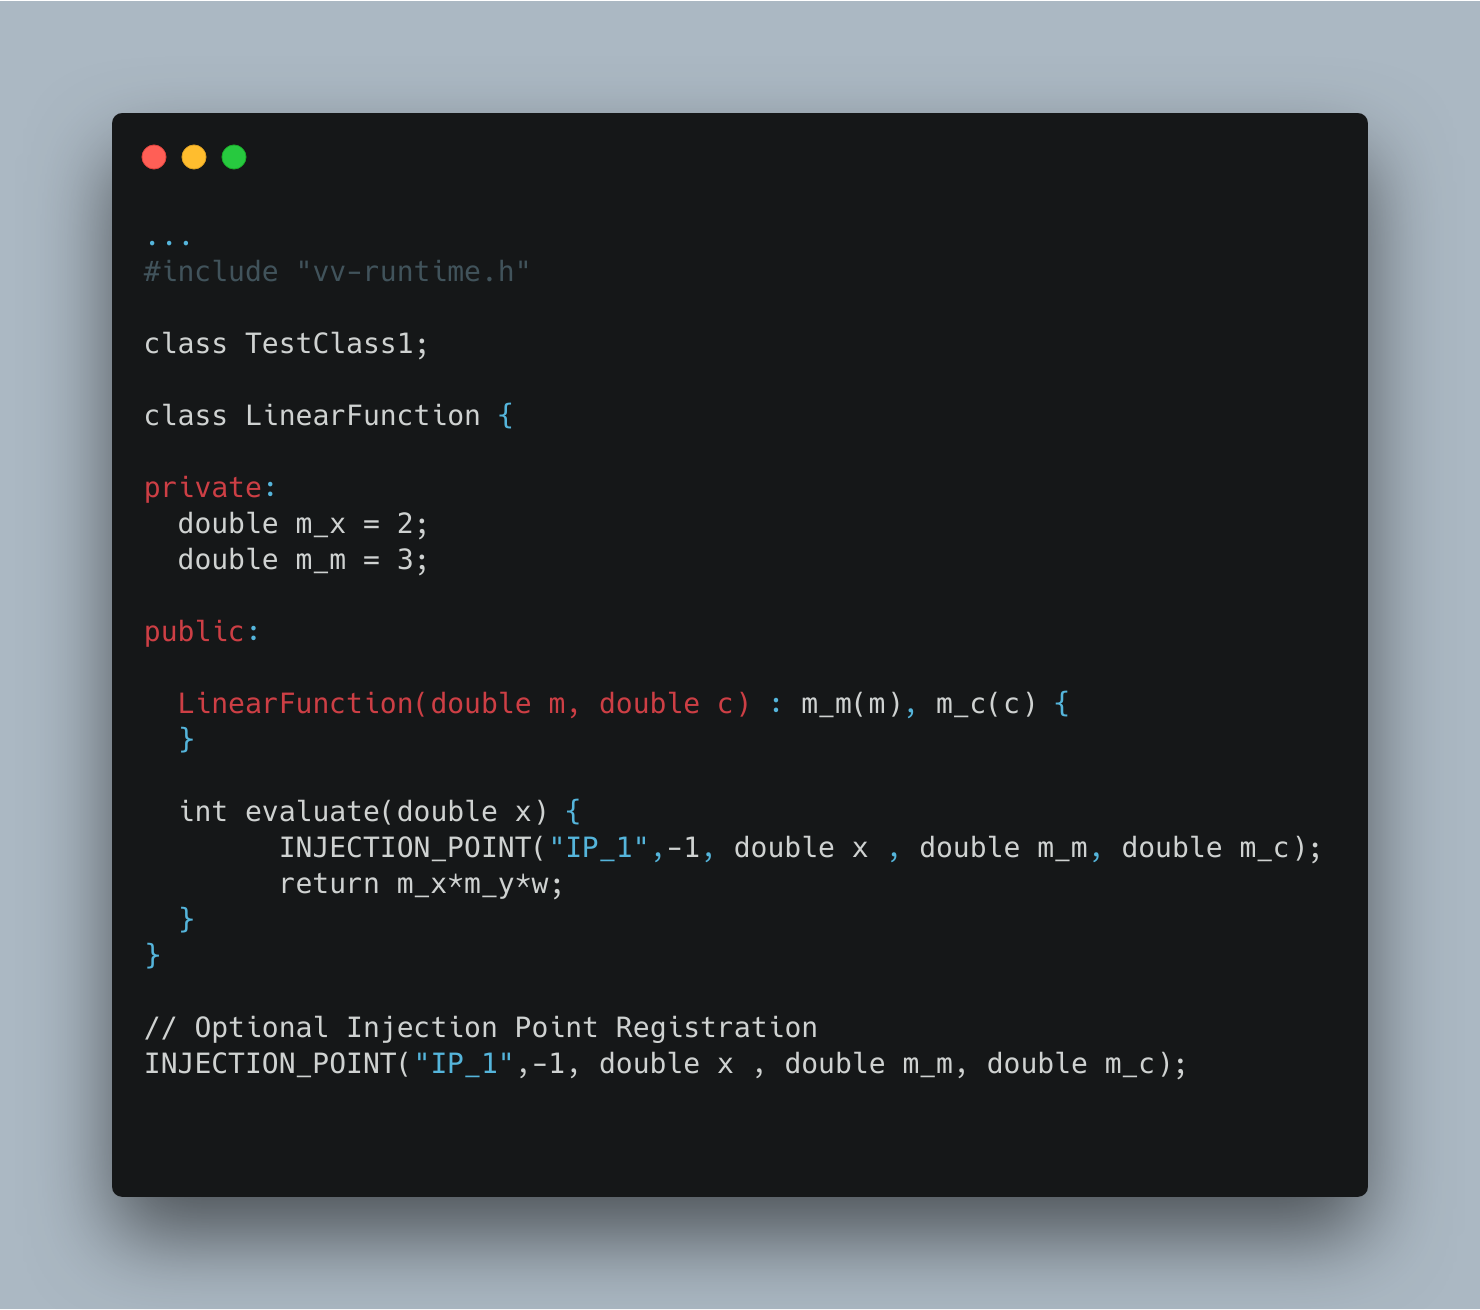
\includegraphics[width=0.45\textwidth]{./Figures/linear.png}
  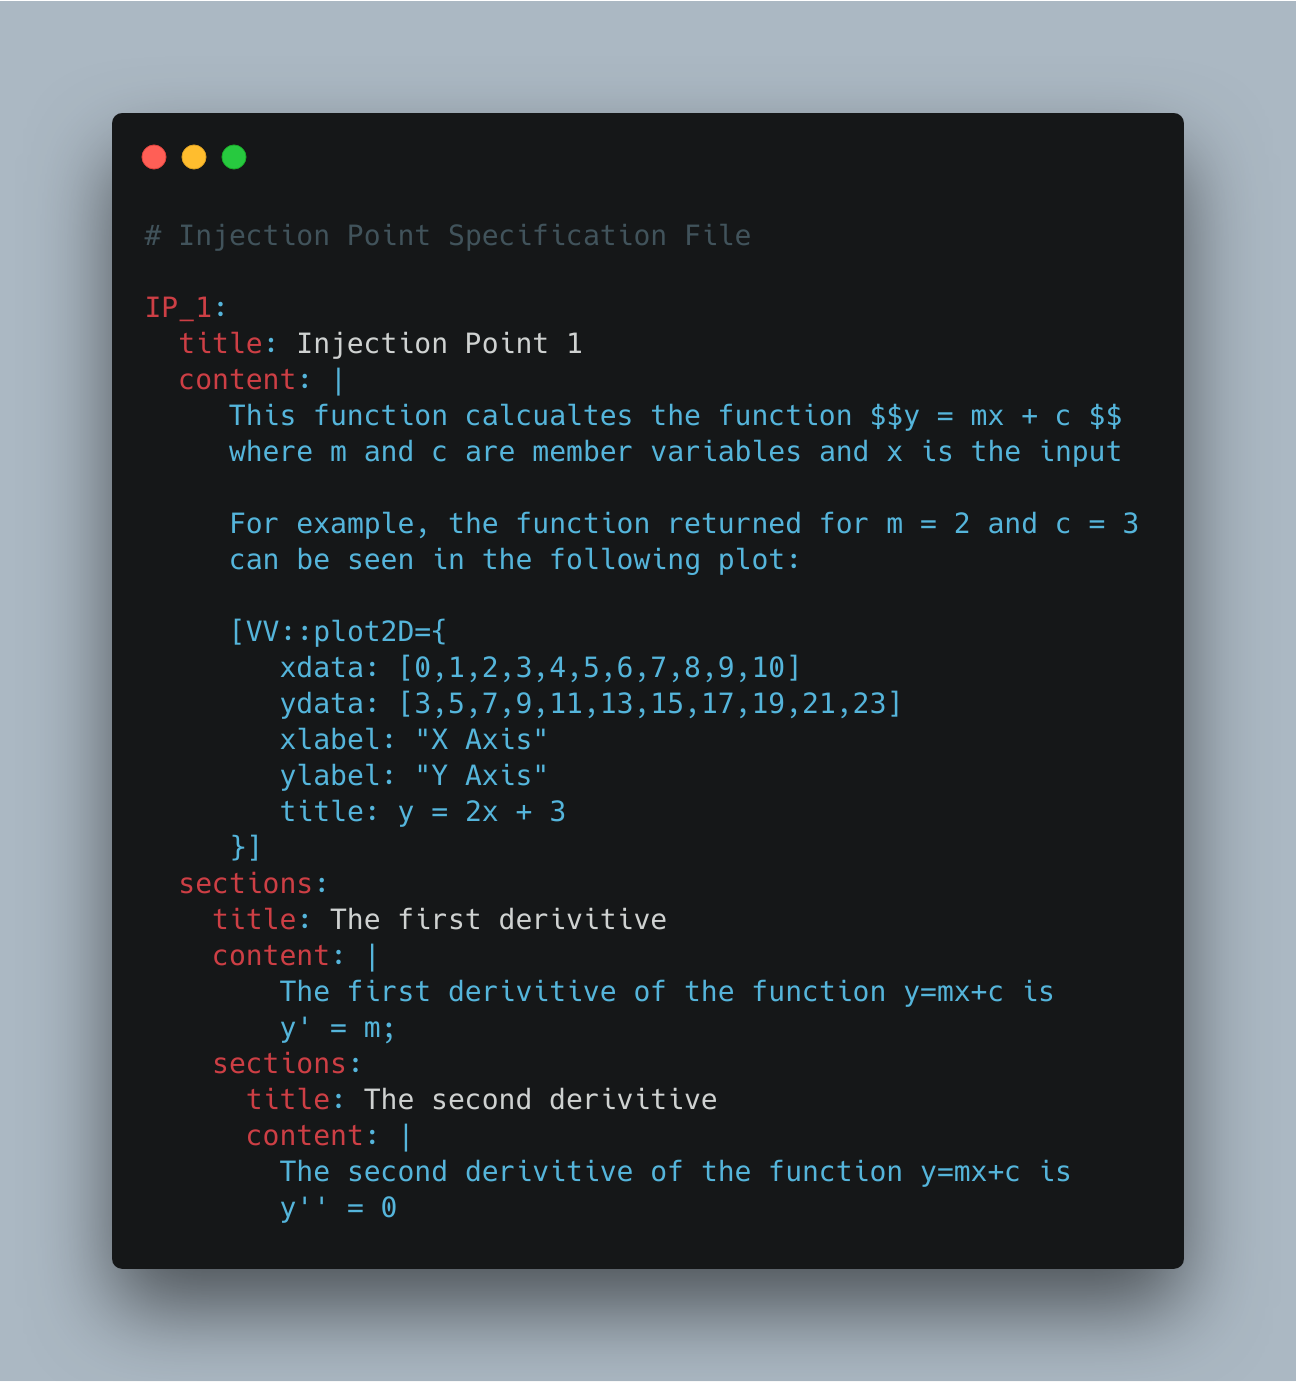
\includegraphics[width=0.45\textwidth]{./Figures/yaml.png}
 \caption{Left: A code Snippet showing a member function enhanced with a single stage injection point. Right: The injection point
 specification describing the state of the code at the injection point. \label{fig:linearEx}
\end{figure}


In C++ codes, the developer can also opt to pre-register the injection point with the runtime module using the REGISTER\_IP macro. The macro uses a feature of object orientated programming languages that allows code in the constructors of static variables to be executed prior to the main function. In this way, one can register certain code elements by simply defining a static variable. Self registration is particularly nice because it allows for run-time detection of the injection points present in the call-graph. That information allows for the automatic generation of a customized test configuration file for each executable. All calls to the REGISTER\_IP macro should be made outside of function calls and classes, as shown in the last line of the code snippet in Figure~\ref{linearEx}. 

Unfortunately, static variables can only be initialized with constant expressions known at compile time in C and FORTRAN, so instead, information about injection points must be determined either by running the full simulation, or by pulling information from the injection point specification files. The custom compiler extension developed in Phase II will address this issue by hardwiring information about the included injection points into the meta-data of the executable or library. 

After an injection point has been declared and optionally registered, the final step is to write the injection point specification. This is specification is used to populate the content of the final \VV report for each simulation. As shown in Figure~\ref{fig:linearEx}, the specification is a YAML file containing a description of the injection point. Writing a YAML specification 
for an injection point is not required; however, the more information entered here, the more informative the final report will be. The fields supported in the YAML specification are:

\begin{itemize}
 \item {\bf title:} A descriptive title for the injection point 
 \item {\bf content:} A markdown formatted string representing the content to be displayed for this injection point in the final report.
 \item {\bf sections:} A map containing the content for any subsections to be displayed under the original content description. Each subsection is displayed  as a collapseble child or its parents content panel and is included in the overall index of the final report. 
 \end{itemize}

The injection point specification is used during report generation, but is not required when running the executable. This
allows the user to fully customize the final report, even after the \VV testing has been completed. Moreover, the content
component of the specification supports a custom extension of the markdown language that allows for automated generation
of a number of custom data visualization components (described below). 

\subsection{The Testing Interface} 

The second facet of the framework is the \VV testing interface. The development of the 
test interface was based on the idea that tests should be loaded at runtime and defined independently of the source code. To achieve this, the test
interface was built using an C++ plugin pattern. This pattern allows users to develop tests is separate testing modules that can be loaded and configured 
at runtime using an XML configuration file. This allows the users to add or remove tests from injection points located in any linked library without ever 
needing to recompile the executable or any of the libraries. 

The first step in the development of a new VnV test is to create a testing library. The framework includes a library generation script that will automatically build the directory structure and makefiles required to 
build this library. Once the library has been initialized, the user can begin to develop individual tests. 

To simplify the process of writing tests, the VnV framework includes a test generation this script. If the library generation script was used, this script will be available in the src directory of the new testing library. To run this script, the user should provide a unique name for the test and a list of the names and types of parameters that will be supported by the new Test. Using this information, the script generates all the boiler plate code required to implement the IVVTest interface and to handle all the required type-casting. 

From this point, completing the test requires the developer to implement two functions; the delcareIO function and the run\_tests function. 

The declareIO function gives the developer an opportunity to pre-declare the IO variables that will be written by the test. These declarations are not required; however, they allow for optimization in the handling of meta-data in the underlying ADIOS2 IO engine. Readers should look to the ADIOS2 documentation for a detailed description on how to set up and declare IO variables. 

The main function of the test is the runTests function. As shown in Figure~\ref{TODO}, the declaration for this function is

\begin{verbatim}
 TestSuccess run_tests(adios2::Engine &engine, int testStage, <type>* <name>, <type>*, <name>,...)
\end{verbatim}

Here, testStage is an integer representing the stage that the test is currently in. A test can support as many stages as there are integers. For example, 
the test shown in Figure~\ref{TODO} supports three stages; one for setup, one for data collection and one for finalization. As will be shown below, the test 
stages are mapped to injection point stages at runtime using the test configuration file. 

Data output can occur at any point in the run\_tests functions. The core runtime module ensures that each test stage is completed in a unique ADIOS2 step. This allows for efficient 
compartmentalization of the test output and makes post-processing significantly easier. As in the delcareIO function; data output is completed directly in ADIOS through the 
ADIOS2 read/write API. As an example, the test in Figure~\ref{TODO} writes a data array to the output during the finalization stage of the test. 

The final step in writing a test is to write the test specification. As with injection points, this specification acts as a template for the 
content to be shown in the final report. The specification is written in a YAML file and supports writing content using the VnV extended markdown format. As will be described 
in the following section, this extended markdown specification allows for direct querying of the data output during each stage of a \VV test. In this way, the user can 
create a generic, data agnositc template for the \VV test output that will be populated with data during post-processing. 

\subsubsection{Variable Modifiers}

In addition to tests, the VnV framework also provides support for pluggable variable modifiers that can be used to 
map injection point parameters into formats that can be consumed by the tests. These Test modifiers are developed using 
the same plugin based C++ pattern used to define the tests and can be included in seperate Modifier libraries or as seperate 
components in existing testing libraries. Some examples of modifiers implemented during the Phase I testing include; a dereference modifier
that dereferences a pointer variable; an array access modifier that pulls out the $n$'th element from an array variable; and a PETScPC modifier that
uses the KSPGetPC function to provide direct access to the internal preconditioner. 


\subsection{Extended Markdown Format for Numerical Simulations} 

The Extended markdown format for numerical simulations, MD-XNS,  was developed for the VnV project as a highly customizable system for automatically processing the results obtained from numerical simulations into interactive, informative HTML/JS web pages. The extension itself was built using py-markdown, an open source python library for converting markdown files into html.

In addtion to standard markdown commands, the MD-XNS format supports custom post-processing commands of the form [VV::<name>={...}], where name is the name of the component the user would like to insert and {...} represents a dictionary of configuration options. 

The Phase I prototype supports a range of custom processing functions including 
\begin{itemize}
\item Table: The table command inserts an interactive, sortable, searchable table into the final html document. The user can populate the table by entering the information
manaully, by providing the name of a csv file, and/or by providing a list of numpy arrays. 
\item Chart2D: The Chart2D command inserts an interactive Charts.JS chart into the document. The entire array of Charts.JS charts are available through this component, including bar, 
line, scatter and pie charts. In each case, the chart is configured using a python dictionary entered directly into the markdown. 
\item VTPView: The VTPView command uses VTK.js to insert interactive 3D visulization of a .VTP files in the final document. 
\item PostPro: The PostPro function allows the user to set up post-processing scripts for execution during the report generation phase. In this way,
users can write simple scripts that parse the data into formats more suitable for use in any of the other data visualization components. 
\item ThreeJs: The ThreeJS command provides another approach for integrating three dimensional visualization in the final report, in this case using three.js for rendering. This 
component is particularly usefull for viewing meshes. 
\end{itemize}

Figures~\ref{TODO} show examples of the html web-components supported using the MD-XNS format. The key functionality of the MD-XNS format lies in its ability to directly interact with data stored in ADIOS2 bp3 steps. For example, Figure~\ref{TODO} shows a MD-XNS file that automatically populates a plot using an array available at an ADIOS2 step under the variable name ``data''. In this way, MD-XNS allows users to write generic templates that can be populated with data during processing. This is particularly nice for \VV injection points and \VV tests because each test knows extactly what data can appear during each call to the overall testing algorithm. 


\subsection{The VnV Runtime Module}

The VnV runtime module is the driving force behind the framework. This module contains all the functionality required  to detect the injection points, parse the
configuration file, setup the ADIOS IO engine, load the external testing libraries and run all the tests. Despite this, configuring a simulation to use the VnV 
framework is a simple, four step task; (1) include the header file, (2) Call the VVInit(<input-file>) function at the start of main, (3) Call the VVFinalize function
before exiting, and (4) link the VnV library to the main library along with any required sublibraries. 

Once the configuration has been completed, users will be able to control the entire VnV process through the input file. The Phase I prototype 
uses a XML based input file. Figure~\ref{TODO} shows the XSD specification for the input file. The VnV toolkit uses a  modified version of Xsd2Cpp to generate 
a C/C++ DOM parser for the XML file. 

The key sections of the input file specification are:
\begin{itemize}
 \item The Simulation Information. The simulation information section is where the user can provide information at the simulation. 
 \item The Testing Libraries. The testing libraries element is used to define external testing libraries that will be used in the final executable. 
 \item The Introduction. The introduction element a
\end{itemize}

\subsubsection{Automated Report Generation}

In addition to the injection point system, the project team also developed an initial prototype for automatically generating
the final report. After accessing the strengths and weaknesses of multiple different approaches, the project team
decided on a server-less HTML/JS format generated using a custom extension of the markdown format. The primary benefit of this approach is portability - the report can be displayed in any web browser - but other benefits include interactive components, non-linear data presentation and high levels of customization. Moreover, the server-less nature of the HTML web-page allows for direct publication on any static web hosting service (github.io, AWS S3, etc.). 

Figures~\ref{TODO} show screen-shots of a sample VnV report generated using a set of toy testing libraries. The main layout consists of three components; the carousel, the index and the content. The carousel is an optional component that can be used to highlight important results of the simulation. It accepts up to ten pictures, each with its own custom caption. Simpler static headers are also possible. The index and content are generated automatically based on the VnV output file. Each node in the index represents an injection point encountered during the simulation. As such, this index represents a coarse grained view of the simulations call stack. At the top of each injection point section is the injection point content as specified in the injection point specification. Following this is the output of each test completed at the injection point. Last is the list of children. These children represent injection points that were initialized between the first and last step of a staged injection point. A live version of this sample VnV report will be available at http://www.rnet-tech.net/VV/sample.html until the date of award notification. 

\subsubsection{ Demonstration in a Moose Application } 
To demonstrate the utility of the method, the project team placed several injection points 
in the main function of a MOOSE example ``ex01'', one injection point in the PETSc Initialize function and 
one injection point in the PETSc Finalize functions. This is an extremely simple example that 
did not test the full limits of the new API; however, it did act to verify that the phase I prototype 
can be used to can be used to perform in-situ verification and validation in a across multiple libraries 
through a single interface. A screenshot of the final \VV report obtained from those tests is shown in the 
final report. 

In summary, during Phase I, the project team created a functioning prototype of the VnV framework that provides:
\begin{itemize}
 \item A clean mechanism for inserting injection points in existing codes
 \item A simple interface for defining custom tests 
 \item A customizable approach for automatic post-processing of testing data and injection points
 \item A python based report generation code that automatically creates an interactive server-less web report based on the VnV output.
\end{itemize}

As will be described in the workplan, the goal of the Phase II project will be to take this initial prototype and extend, harden and 
optimize it such that it can be efficiently used in high performance computing applications. 

\section{Phase I Task Completion}
With regard to the proposed Phase I tasks, our achieved objectives are as 
follows:

\subsection{Task 1: }


\subsection{Task 2: }


\subsection{Task 3: }

\section{Summary and Conclusions}

During Phase I of the project, RNET have tackled various technical 
challenges with regard to developing a modern framework for facilitating 
in-situ end-user verification and validation in general purpose numerical 
simulation packages.  This capability, when fully 
developed, will provide a convenient interface for creating explainable numerical 
simulations that not only provide the user with a solution, but also a detailed 
report on how the solution was obtained and why it should be trusted. 

In order to demonstrate 
feasibility of developing this product, RNET has accomplished the 
following.

\begin{itemize}
 \item Developed cross library support for defining and registering injection points in general purpose numerical simulation packages.
 \item Created an interface for writing and integrating custom V\&V tests that can be configured at runtime.
 \item Developed a custom markdown format that allows for automated post-processing and visualization of testing data.
 \item Implemented an automated documentation generation script that creates a server-less, interactive VnV report that can be 
 displayed in any web browser. 
 \item Demonstrated how the VnV reports could be viewed in the NEAMS workbench through the QWebEngineView. 
\end{itemize}

The above evaluations demonstrate the technical feasibility of the proposed 
approach.  This 
platform also has great commercial potential. RNET intends to promote 
the VnV framework by initially supporting relevant open-source computational tools to 
leverage their existing customer base. 


\section{Publications and Presentations}
None




\bibliography{bib/proposal.bib}

\end{document}
